\subsection{Teorema de \vank}
Este teorema es considerado como el mas útil a la hora de hacer
identificaciones de grupos fundamentales. Su idea se basa en que si
tenemos un espacio \(X\) y dos subconjuntos \(U,V\) tales que \(X = U
\cup V\), entonces podemos estudiar el grupo \(\pi (X, x_0)\) como un
subgrupo del grupo libre generado por \(\pi (U, x_0)\) y \(\pi (V,
x_0)\) si \(x_0 \in U \cup V\). Para obtener un isomorfismo tomamos un
cociente adecuado. El caso mas claro de aplicación se vera que son para
las \emph{wedge sum} en donde este cociente sera trivial. En casos mas
generales se vera que el cociente es de una forma relacionada con la
definición de producto libre. Procedemos para iniciar la definición de
estas.

\begin{definicion}[Producto libre]
  Sea \(G_\alpha\) una colección de grupos. El grupo libre \(*_\alpha
  G_\alpha \) consiste como conjunto en todas las cadenas reducidas
  \[ g_1 g_2 g_3 \dots g_m \]
  para \(m \geq 0\) arbitrario tal que todo \(g_i\) pertenece a
  \(G_{\alpha_i}\), \(g_i\) sea distinto de la identidad de
  \(G_{\alpha_i}\) y índices sucesivos son distintos, ie \(\alpha_i \neq
  \alpha_{i + 1}\). Tomando la identidad como la cadena vacía y como
  operación de grupo la juxtaposicion de cadenas
  \[ (g_1 g_2 \dots g_m ) * (h_1 h_2 \dots h_l) = g_1 g_2 \dots g_m
    h_1 h_2 \dots h_l \]
  en donde se debe reducir la cadena para que términos seguidos no
  pertenezcan al mismo grupo.
\end{definicion}
\begin{acotacion}
  Es claro que la cadena vacía es la identidad. Para ver la inversa de
  una cadena nos basamos en el proceso de reducción. Sea \(g_1 g_2 \dots
  g_m\) una cadena arbitraria, su inversa corresponde a \(g_m^{-1} g_{m-1}^{-1}
  \dots g_1^{-1}\) pues
  \begin{gather*}
    g_1 g_2 \dots \underbrace{g_m g_m^{-1}}_{= e_{\alpha_m}}
      g_{m-1} \dots g_1^{-1} \\
    = g_1 g_2 \dots g_{m-1} \dots g_1^{-1}
  \end{gather*}
  donde la identidad fue removida de la cadena por el requisito de ser
  una cadena reducida. Si este proceso continua iterativamente se
  obtendrá la cadena vacía que es la identidad.

  Por otro lado se nota que no hay requerimiento de que todos los grupos
  participen en todas las cadenas. De hecho, todos los elemento de
  cualquiera de los grupos participantes \(G_\alpha\) pertenecen al
  conjunto de cadenas reducidas como cadenas con \(m = 1\) y indice
  adecuado.
\end{acotacion}
Esta construcción puede considerarse como una alternativa a \(\prod
G_\alpha\) o \(\oplus G_\alpha\) en donde elementos de distintos grupos
no conmuten entre si. Algo que no es claro sobre este grupo es si
su operación es asociativa, esto lo probaremos en el siguiente teorema
por completitud
\begin{teorema}
  El producto de \(*_\alpha G_\alpha\) es asociativo.
\end{teorema}
\begin{proof}
  Mostrar directamente la asociatividad del producto seria un ejercicio
  de enumerar los casos donde puede ocurrir un reducción de cadena.
  Nosotros seguiremos una vía alternativa dada por \emph{Hatcher} en
  \cite{Hatcher}[sec 1.2] de estudiar la cada posible juxtaposicion como
  una función en el espacio de permutaciones. Sea \(W\) el conjunto de
  cadenas reducidas de \(*_\alpha G_\alpha\) con la cadena vacía
  incluida. Para cada \(g \in G_\alpha\) se define una función asociada
  \(L _g : W \to W\) dada por la ecuación
  \[ L_g \left( g_1 g_2 \dots g_m \right) = g g_1 g_2 \dots g_m \]
  con \(g g_1\) reducido si \(g_1 \in G_\alpha \) para mantener que sea
  una cadena reducida en \(W\). Una propiedad clara es que podemos
  reducir antes o después de asociar \(L\) y no afectara el resultado,
  dicho formalmente sea \(g, g', \hat g \in G_\alpha\) con \(\hat g = g
  \cdot g'\). La asociación \(L_{g g'} = L_{g} \circ L_{g'}\) pues para
  una cadena arbitraria
  \begin{align*}
    &L_{g g'} \left( g_1 g_2 \dots g_m \right) \\
    &= (g g') (g_1 g_2 \dots g_m) \\
    &= (\hat g) (g_1 g_2 \dots g_m) \\
    &= (g (g' (g_1 g_2 \dots g_m))) \\
    &= L_g \circ L_{g'} \left( g_1 g_2 \dots g_m \right)
  \end{align*}
  notando de que en el caso que \(g_1 \in G_\alpha\) se tiene un
  reducción intermedia. Se ve también de todo \(L_g\) con \(g \in
  G_\alpha\) tiene una asociada inversa \(L_{g^{-1}}\) con \(g^{-1} \in
  G_\alpha\), lo cual en consecuencia nos da un mapeo de identidad a
  identidad (por regla de reducción). Tenemos en cierto sentido un
  homomorfismo de grupos, solo que dado que no conocemos la
  asociatividad de la juxtaposicion, el espacio de partida no seria
  grupo. Sin embargo ambas operación están relacionadas mediante la
  formula
  \begin{align*}
    G_\alpha &\longrightarrow P(W) \\
    g &\longmapsto L_g
  \end{align*}
  donde \(\left( W \to W , \circ \right) = P(W)\) el grupo de
  permutaciones (ie ya no solo viendo \(L_g : W \to W\)). Podemos
  generalizar esta asociación en su primer argumento a todo \(W\) por
  \begin{align*}
    L : W &\longrightarrow P(W) \\
    g_1 g_2 \dots g_k &\longmapsto L_{g_1} \circ L_{g_2} \circ \dots
    \circ L_{g_k}
  \end{align*}
  así es claro que una operación juxtaposicion en \(W\) es una
  composición en \(P(W)\). Esto obliga a que la juxtaposicion sea
  asociativa pues por contradicción, si tuviéramos un trio de términos
  \(w_1, w_2, w_3 \in W\) cuya juxtaposicion no fuera asociativa, implicaría
  que bajo la asociación anterior, la composicion de \(L_{w_1}, L_{w_2},
  L_{w_3}\)tampoco lo seria, lo cual es una contradicción con la
  asociatividad de la composición en \(P(W)\).
\end{proof}

Aquí se utilizo implícitamente un propiedad básica del producto libre
\(*_\alpha G_\alpha\), que si tengo una colección de homomorfismos
\[ \phi_\alpha : G_\alpha \to H \]
con \(H\) un grupo, existe una extensión única
\[ \phi : *_\alpha G_\alpha \to H \]
tal que sigue siendo homomorfismo. En particular, la ecuación que la
define para \(g_1 g_2 \dots g_n \in *_\alpha G_\alpha\) arbitrario es la siguiente
\[
  \phi \left( g_1 g_2 \dots g_n \right) := \phi_{\alpha_1} (g_1)
  \phi_{\alpha_2} (g_2) \dots \phi_{\alpha_n} (g_n)
\]
Para probar que es única, basta notar reducir la cadena no afecta la
imagen bajo \(\phi\) y que esta debe seguir siendo un homomorfismo.

El marco de trabajo de \vank sera el siguiente diagrama conmutativo,
\begin{figure}[h]
  \centering
  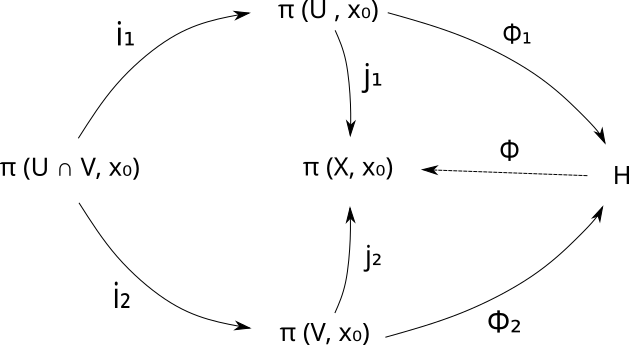
\includegraphics[scale=0.5]{./imagenes/van.png}
\end{figure}
donde \( H = \pi (U, x_0) * \pi (V, x_0)\) el producto libre, \(i_1,
i_2, j_1, j_2\) son los homomorfismos inducidos (sin la notación \(i_*\)
por simplicidad) de las inclusiones correspondientes, \(\Phi_1, \Phi_2\)
son las inclusiones en el grupo libre tomando todo \(\gamma \in \pi (U,
x_0)\) y ver la correspondiente cadena \(\gamma \in H\) y \(\Phi :
\pi(U, x_0) * \pi (V, x_0) \to \pi (X, x_0)\) la extensión de los
homomorfismo \(\Phi_1, \Phi_2\) descrita en el párrafo anterior.

Previo al teorema general, es útil trabajar con una versión reducida del
teorema de \vank por dos razones: es una versión geométricamente
intuitiva y aparece como paso intermedio de la demostración general.

\begin{teorema} \label{thm:vank-especifico}
  Sea \(X = U \cup V\), donde \(U,V\) son conjuntos abiertos de \(X\).
  Supongamos que \(U \cap V\) es arco-conexo y que \(x_0 \in U \cap V\).
  Sea \(j_1\) y \(j_2\) las inclusiones de \(U\) y \(V\) en \(X\)
  respectivamente. Entonces las imágenes de los homomorfismos inducidos
  \[ j_{1,*} : \pi (U, x_0) \to \pi (X, x_0) \quad j_{2,*} : \pi
  (V, x_0) \to \pi (X, x_0) \]
  generan a \(\pi (X,x_0)\)
\end{teorema}
\begin{proof}
  Hemos de probar que para todo arco \(f\) en \(X\) basado en \(x_0\),
  es arco-homotopico a un arco de la forma
  \[ g_1 * g_2 * ... * g_n \]
  donde cada \(g_i\) es un arco en \(X\) basado en \(x_0\) que esta
  contenido completamente en \(U\) o en \(V\).

  Para esto, mostramos que existe una subdivisión de \(I\) dada por
  \(a_0 < a_1 < ... < a_n \) tal que \(f(a_i) \in U \cap V\) y que \(
  f([a_i , a_{i+1}]) \) es subconjunto contenido solo en \(U\) o en
  \(V\).

  Por lema \ref{thm:lebesgue-number-lema} (numero de Lebesgue),
  existe una subdivisión de \(I\) dada por \(b_1 < ... < b_n\) tal que
  \(f ([b_i , b_{i+1}])\) pertenece completamente a \(U\) o \(V\) para
  todo \(i \in [1,n]\). Si para para todo \(i\) se cumpliera que
  \(f(b_i) \in U \cap V\) hemos terminado. En caso contrario, de existir
  \(i\) tal que \(f(b_i) \not \in U \cap V\) esto implica que
  \[ f(b_i) \in U \ \veebar \ f(b_i) \in V \]
  Tomando s.p.d.g la primera alternativa, implicaría que
  \[ f(b_i) \in U \implies f([b_{i-1}, b_{i}]) \subset U \ \land \ f([b_i,
    b_{i+1}]) \subset U \]
  Análogamente si \(f(b_i) \in V\). Podemos olvidar entonces el valor
  \(b_i\) de la subdivisión y revisar si \(f(b_{i+1}) \in U \cap V\),
  repitiendo este proceso una cantidad finita de veces hasta satisfacer
  la condición.

  Ahora se prueba el teorema en si. Dado \(f\) y \(a_0 < ... < a_n\)
  subdivisión anterior, definamos las funciones
  \[ l_i : [0,1] \to [a_{i-1}, a_{i}] \]
  \[ f_i = f \circ l_i \]
  Es claro que \(\forall i \in [1, n], \ f_i (I) \) esta contenida en
  \(U\) o en \(V\). También es claro por simple calculo que se cumple
  que
  \[ [f] = [f_1] * [f_2] * ... * [f_n] \]
  Pero estos \(\{f_i\}\) no son arcos cerrados basados en \(x_0\) de
  \(\pi (U,x_0)\) o \(\pi (V,x_0)\). Para solucionar esto, nos basamos
  en la arco conexidad de \(U \cap V\), lo que nos permite afirmar que
  para todo \(i \in [1 , n]\) existe
  \[ \alpha_i : I \to U \cap V \]
  \[ \alpha_i (0) = x_0 \quad \alpha_i (1) = f(a_i) \]
  arcos continuos, fijando además \(\alpha_0 \equiv x_0 \equiv \alpha_n
  \). Estos nos permiten construir los arcos
  \[ g_i = \alpha_{i-1} * f_i * \alpha_i^{-1} \]
  los cuales si están basados en \(x_0\), y cuya imagen sigue estando
  contenida en \(U\) o en \(V\). Por simple calculo se ve que
  \[ [g_1] * ... * [g_n] = [f_1] * ... * [f_n] = [f] \]
\end{proof}
\begin{corolario}\label{cor:sobre-van}
  El homomorfismo \(\Phi : \pi (U, x_0) * \pi (V, x_0) \to \pi (X,
  x_0)\) es sobreyectivo.
\end{corolario}
Uno puede generalizar el teorema anterior para una cantidad arbitraria
de conjuntos \(A_\alpha\) tal que \(X = \bigcup A_\alpha\). La
demostración es la misma, solo tal vez un poco mas difícil de
visualizar. Lo importante de este teorema es el corolario, el cual
utilizaremos en su forma generalizada para probar el teorema general.

\begin{teorema}[Teorema \vank ]
  Sea \((X, x_0)\) un espacio puntuado tal que exista una familia de
  conjuntos \(\{A_\alpha\}_{\alpha \in \tau}\) tal que \(\forall \alpha
  \in \tau,\ x_0 \in
  A_\alpha\) y \( X = \bigcup_{\alpha \in \tau} A_\alpha\). Si para cada
  intersección \(A_\alpha \cap A_\beta\) es arco-conexa, entonces el
  homomorfismo
  \[ \Phi : *_\alpha \pi (A_\alpha, x_0) \to \pi (X, x_0) \]
  es sobreyectivo. Mas aun, si cada intersección \(A_\alpha \cap A_\beta
  \cap A_\gamma\) es arco-conexa, entonces el kernel de \(\Phi\) es un
  subgrupo normal \(N\) de la forma
  \[
    N := \langle \{ i_{\alpha \beta} (\omega) * i_{\beta \alpha} (\omega)^{-1}
    \mid \omega \in \pi \left( A_\alpha \cap A_\beta, x_0 \right)\} \rangle
  \]
  y por tanto \(\Phi\) induce un isomorfismo \(\pi (X, x_0) \simeq
  *_\alpha \pi (A_\alpha, x_0) / N \)
\end{teorema}
\begin{proof}
  En el corolario \ref{cor:sobre-van} ya fue probado que \(\Phi :
  *_\alpha A_\alpha \to \pi (X, x_0)\) es sobreyectivo. Solo nos falta
  caracterizar al kernel de \(\Phi\).
\end{proof}
% En un espacio \((X, x_0) = (U \vee V, x_0)\) se cumple por la unión
% disjunta que el único punto en común de \(U\) y \(V\) es \(x_0\) (y eso
% solo por la identificación de la equivalencia). Los espacios singletons
% son trivialmente arco-conexos, lo cual nos permite aplicar el teorema
% anterior para calcular grupos fundamentales de estos.
